\documentclass[9pt]{extarticle}

\usepackage[margin=0.5in,top=0.4in,bottom=0.4in]{geometry}
\usepackage{titlesec}
\usepackage{enumitem}
\usepackage{parskip}
\usepackage{xcolor}
\usepackage{hyperref}
\usepackage{multicol}
\usepackage{graphicx}

\setlength{\columnsep}{18pt}

\definecolor{orncblue}{RGB}{35,55,120}

\titleformat{\section}
  {\normalfont\bfseries\color{orncblue}\normalsize}
  {}{0em}{}
  [{\titlerule[0.6pt]}]

\titlespacing*{\section}{0pt}{3pt}{2pt}

\titleformat{\subsection}
  {\normalfont\bfseries\small}
  {}{0em}{}

\titlespacing*{\subsection}{0pt}{2pt}{1pt}

\setlist[itemize]{
  topsep=0pt,
  itemsep=0pt,
  parsep=0pt,
  leftmargin=1.1em
}

\setlist[enumerate]{
  topsep=0pt,
  itemsep=0pt,
  parsep=0pt,
  leftmargin=1.1em
}

\setlength{\parskip}{2pt}
\pagestyle{empty}


\begin{document}

\begin{center}
{\Large\bfseries\color{orncblue} Dissertation Proposal One-Pager}\\[1pt]
{\normalsize AI/ML-Enabled Microstructure Analysis Pairing for Atom Probe Tomography and Time-of-Flight Secondary Ion Mass Spectrometry}\\[1pt]
{\footnotesize Jose Tupayachi \quad$\vert$\quad September 18, 2026}
\end{center}
\vspace{-4pt}

\begin{multicols}{2}

\section{Dissertation Theme}
% This dissertation develops and validates a shared, multimodal machine-learning framework -- spectral encoder + spatial encoder + cross-attention fusion + scientific-LLM reporting -- that automates ranging, reconstruction disambiguation, and microstructure feature extraction across two correlative nanoscale characterization modalities: Atom Probe Tomography (APT) and Time-of-Flight Secondary Ion Mass Spectrometry (ToF-SIMS). The three papers form an escalating arc: (1) establish the shared framework and demonstrate the manual bottleneck it replaces, (2) automate the two hardest disambiguation steps (ranging and pole indexing), and (3) close the loop with literature-grounded, human-reviewed automated reporting.

This dissertation develops and validates a shared multimodal machine-learning framework, comprising spectral and spatial encoders, cross-attention fusion, and LLM reporting, to automate ranging, reconstruction disambiguation, and microstructure feature extraction across two nanoscale characterization modalities: Atom Probe Tomography (APT) and Time-of-Flight Secondary Ion Mass Spectrometry (ToF-SIMS). The three papers form an escalating research approach: (1) Establish the shared framework and demonstrate the manual bottlenecks it addresses, (2) Automate two of the most challenging tasks, ranging and pole indexing, and (3) close the loop with literature supported reporting.

\section{Background \& Motivation}

APT datasets encode two complementary, modalities: a mass spectrum requiring element/molecular-ion \emph{ranging}, and a reconstructed 3D atom map from which precipitates, boundaries, clusters, and CSRO/CMRO are extracted. \\

Both steps are manual, expertise-dependent, and scale poorly on APT datasets. A demonstrated LAMDA workflow on real data confirms concrete bottlenecks: SEM-coregistered tip-profile calibration, reconstruction parameterization, pole-line indexing returning ambiguous BCC/FCC candidates, and RNG/RRNG ranging of overlapping molecular ions (e.g., Fe/Cr/Ni/Mo oxides and carbides). On the other hand, ToF-SIMS shares the same two-modality structure (spectrum + spatial ion image and accesible via pySPM). This motivates one shared AI/ML framework differing only in instrument-specific ingestion.

\begin{center}
    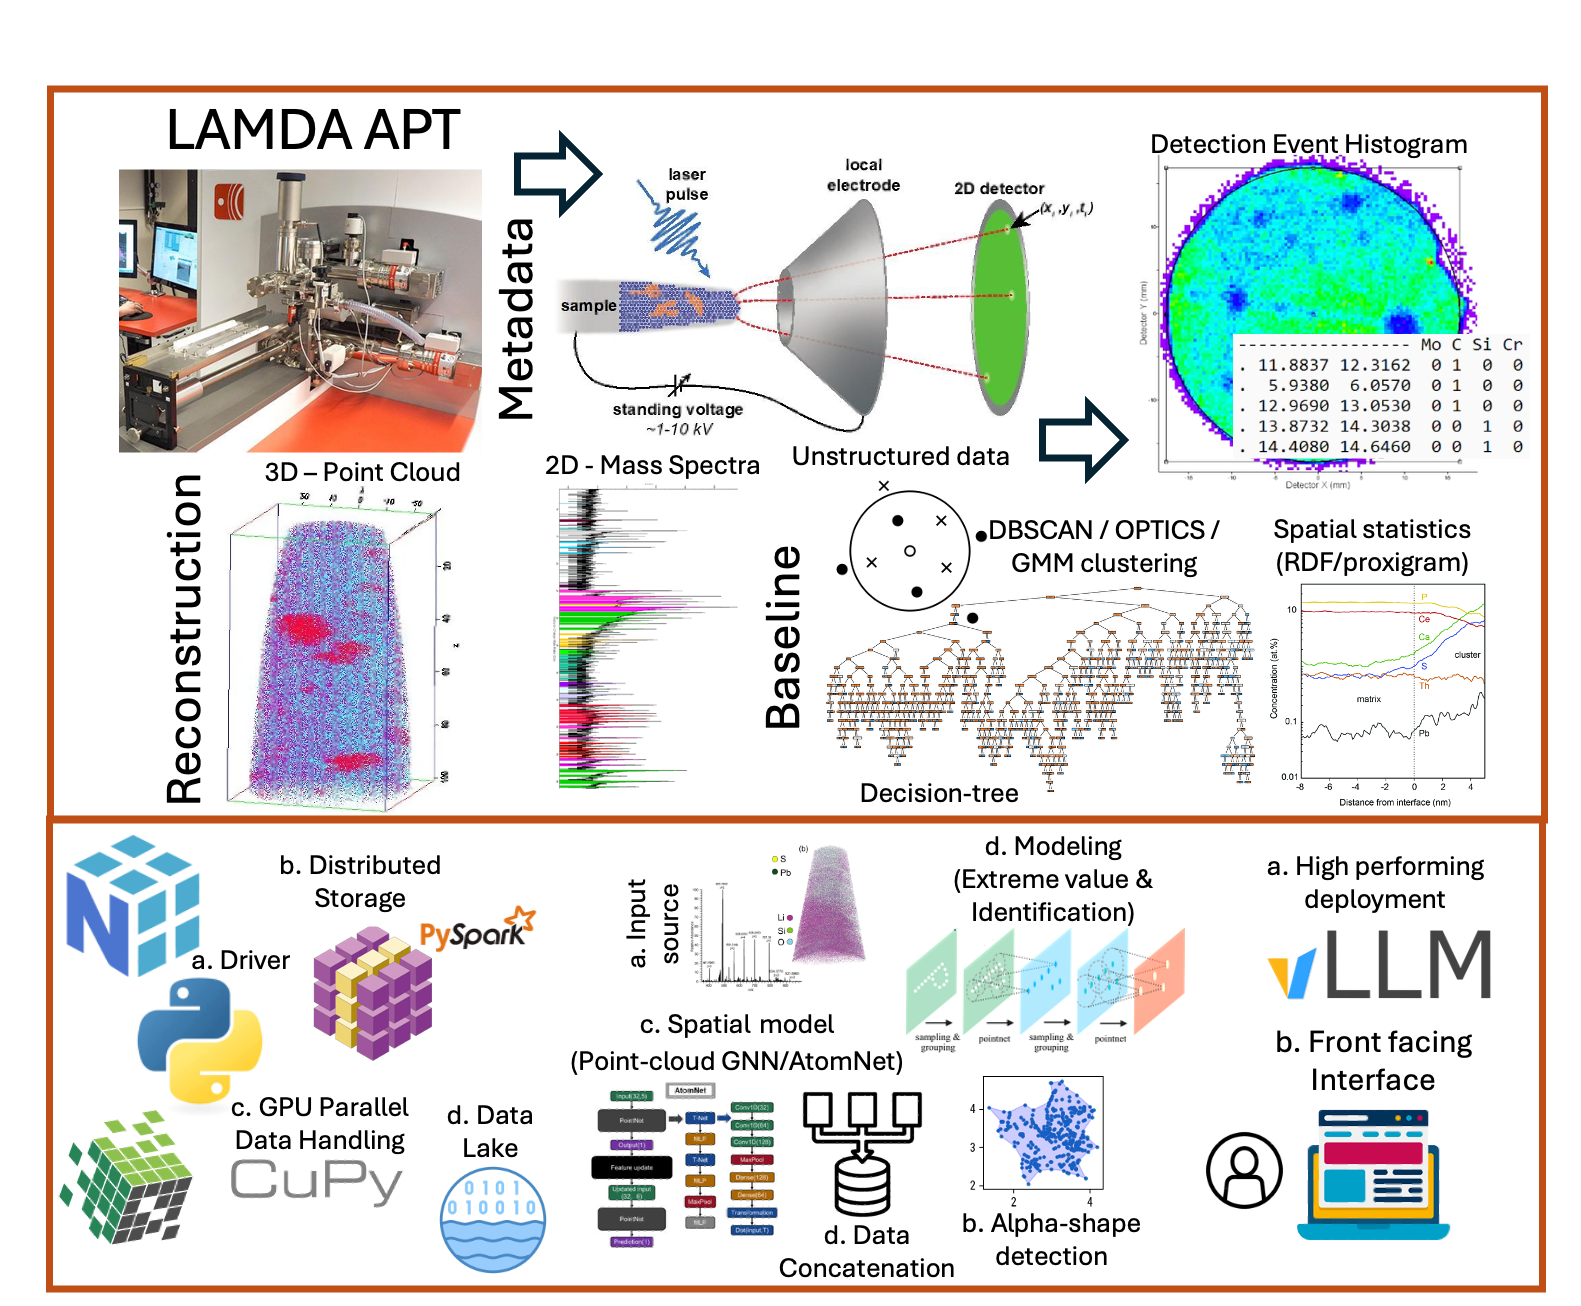
\includegraphics[width=\linewidth]{Main.png}
    
    \small
    \textbf{Figure 1.} Overview of the proposed multimodal AI/ML framework linking spectral and spatial representations exemplifying APT analysis.
\end{center}
\section{Three-Paper Structure}

\subsection{Paper 1 (Basis for Fall proposal defense): A Shared AI/ML Framework for Automated Ranging and Microstructure Screening in APT and ToF-SIMS}
\begin{itemize}
\item Establishes the common two-modality representation and staged framework (spectral encoder + spatial encoder + fusion) shared by APT and ToF-SIMS.
\item Documents the manual baseline and its concrete failure modes on real LAMDA APT data (reconstruction ambiguity, molecular-ion overlap).
\item Defines the FAIR transcoding layer for vendor formats (POS/RNG/RRNG for APT, ITA/ITM/ITS via pySPM for ToF-SIMS) as shared ingestion.
\end{itemize}

\subsection{Paper 2 (Year 2): Automated Multimodal Ranging and Reconstruction via ML-ToF/Bayesian Peak Assignment and Learned Pole Indexing}
\begin{itemize}
\item 1D CNN/transformer spectral encoder for ranging, CNN/GNN spatial encoder for cluster and phase detection, resolves the BCC-vs-FCC pole-indexing ambiguity and molecular-ion overlap identified in Paper 1.
% \item Systematic grid-sweep experiments across model/config combinations to quantify accuracy vs. the manual baseline.
\end{itemize}

\subsection{Paper 3 (Year 3): LLM-Driven Reporting and Literature-Grounded Interpretation for Correlative APT--ToF-SIMS Characterization}
\begin{itemize}
\item Integrates fused spectral/spatial embeddings into a LLM + literature RAG reporting layer.
\item Validates automated reports against expert-authored reports, benchmarks the deployed vLLM pipeline.
\end{itemize}

\section{Committee Formation Plan}
\begin{itemize}
\item Advisor/chair: Dr. Li \& Dr. Yu \& Dr. Yao \& Dr. Das.
% \item Identify 3--4 additional members spanning: APT/materials-science domain expert, ML/AI methods expert, ToF-SIMS/surface-science expert, and a graduate-school/outside-department representative.
% \item Target: Confirm membership before circulating the proposal document; committee finalized well ahead of the Fall defense.
\end{itemize}

\section{Timeline to Fall Proposal Defense}
\begin{itemize}
\item \textbf{Now - 9/18:} This one-pager finalized.
\item \textbf{Sept-Oct:} Finalize Paper 1 draft, internal review.
\item \textbf{October:} Circulate written proposal to committee ($\geq$2 weeks before defense).
\item \textbf{November:} Schedule and defend proposal.
% \item \textbf{Ongoing (parallel):} Finalize CAPARS synoptic-data ML paper; benchmark vLLM + \texttt{ornl-qwen3-8-27b} literature pipeline; update Task 3 framework materials.
\end{itemize}

\end{multicols}

\end{document}
